\documentclass[11pt,a4paper]{article}
\usepackage{graphicx, float}
\usepackage[utf8]{inputenc}
\usepackage{amsmath, amssymb, amsthm}
\usepackage[T1]{fontenc}
\usepackage{lmodern}
\usepackage[english]{babel}
\usepackage{hyperref}
\usepackage{xcolor}
\usepackage{geometry}
\usepackage{fancyhdr}
\usepackage{cancel}
\usepackage[ruled,vlined]{algorithm2e}
\usepackage{tikz}
\usepackage{subcaption}
% ==========================
% Page Setup
% ==========================
\geometry{margin=1in}
\pagestyle{fancy}
\fancyhf{}
\rhead{Daniel Kozin}
\lhead{Diffusion Models}
\cfoot{\thepage}

\begin{document}

% ==========================
% Title Page
% ==========================
\thispagestyle{empty}
\begin{titlepage}
    \centering
    \vspace*{3cm}
    
    {\Huge\bfseries Diffusion Models - Project Proposal \par}    
    \vspace{3cm}
    {\Large Daniel Kozin \par}
    \vspace{1em}
    {\Large ID: 215550260 \par}
    \vspace{3em}
    {\Large \today \par}
    \vfill
\end{titlepage}

% ==========================
% Start Real Content
% ==========================
\pagestyle{fancy}
\setcounter{page}{1} 

\section{Project Proposal}
In my previous research project, I worked with a specialized data set of 3D MRI images of breast phantoms, designed to represent a lump within the breast, as shown in Figure~\ref{fig:phantoms}. In that project, we used a robotic arm to palpate the phantom and learn a representation of the palpation. Using this representation, we trained a model to predict the original phantom structure.
\\\\
It is worth noting that this data set is fairly limited in size: even after augmenting each scan with eight rotations, it amounts to fewer than 800 volumes in total.

\begin{figure}[H]
    \centering
    \begin{subfigure}[b]{0.22\textwidth}
        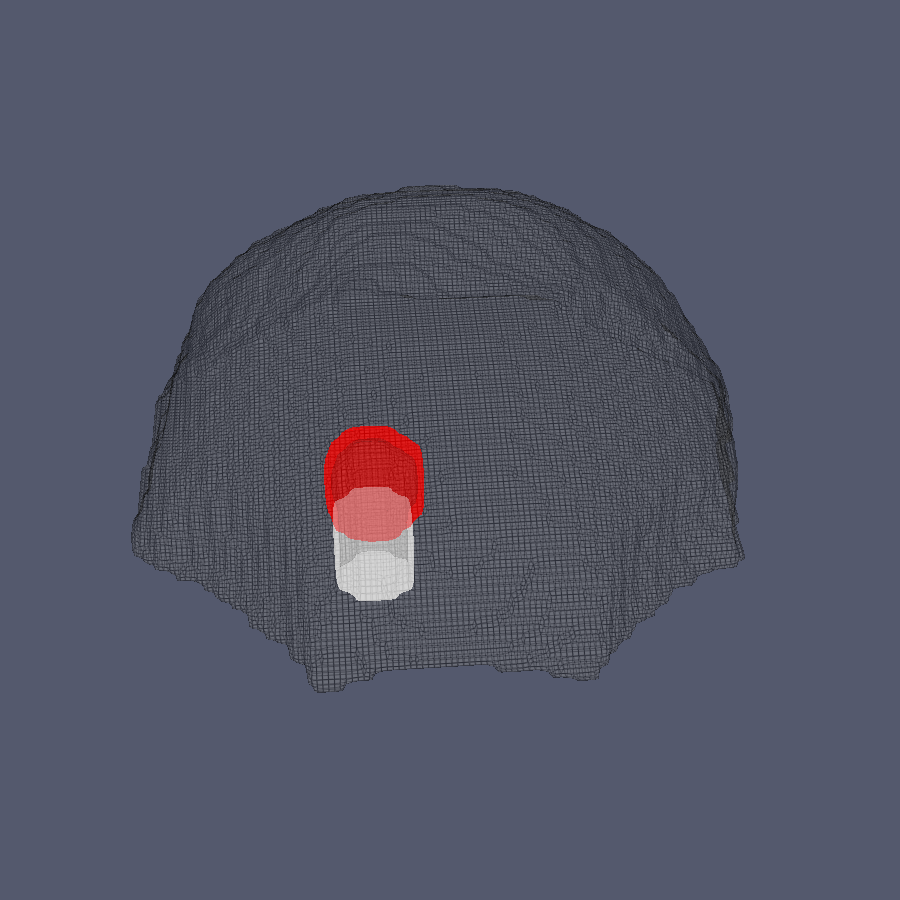
\includegraphics[width=\textwidth]{imgs/showcase_showcase_gt_0.png}
    \end{subfigure}
    \hspace{1em}
    \begin{subfigure}[b]{0.22\textwidth}
        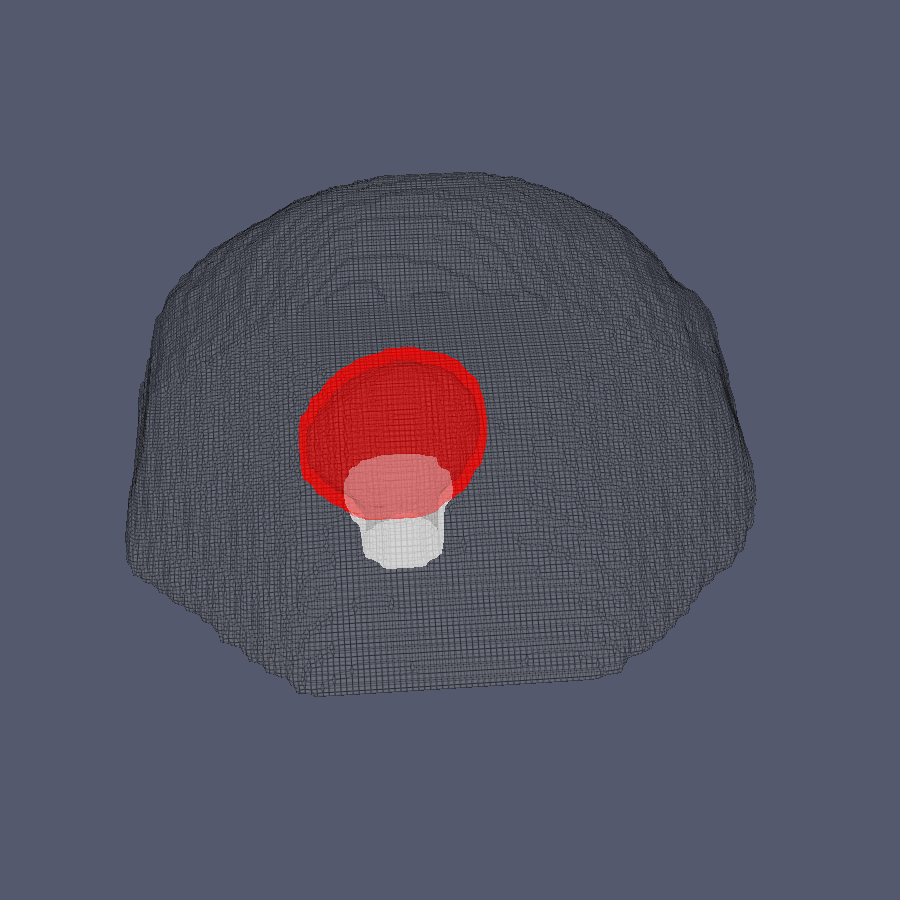
\includegraphics[width=\textwidth]{imgs/showcase_showcase_gt_13.png}
    \end{subfigure}

    \vspace{0.5em}

    \begin{subfigure}[b]{0.22\textwidth}
        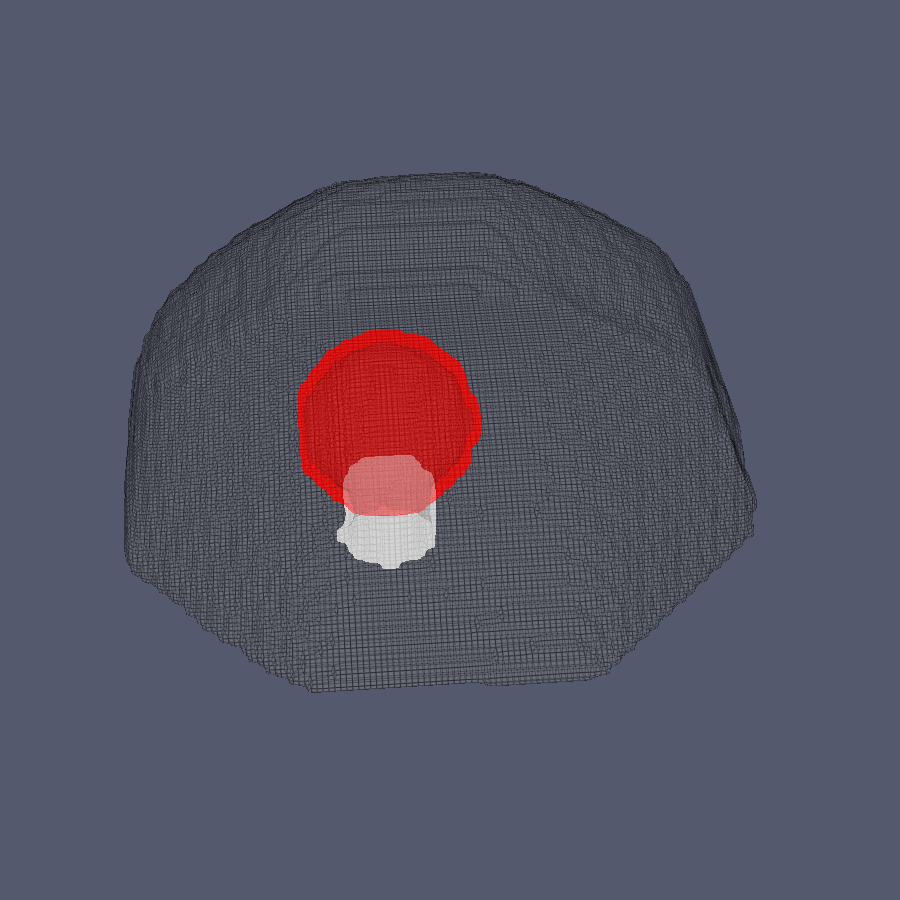
\includegraphics[width=\textwidth]{imgs/showcase_showcase_gt_70.png}
    \end{subfigure}
    \hspace{1em}
    \begin{subfigure}[b]{0.22\textwidth}
        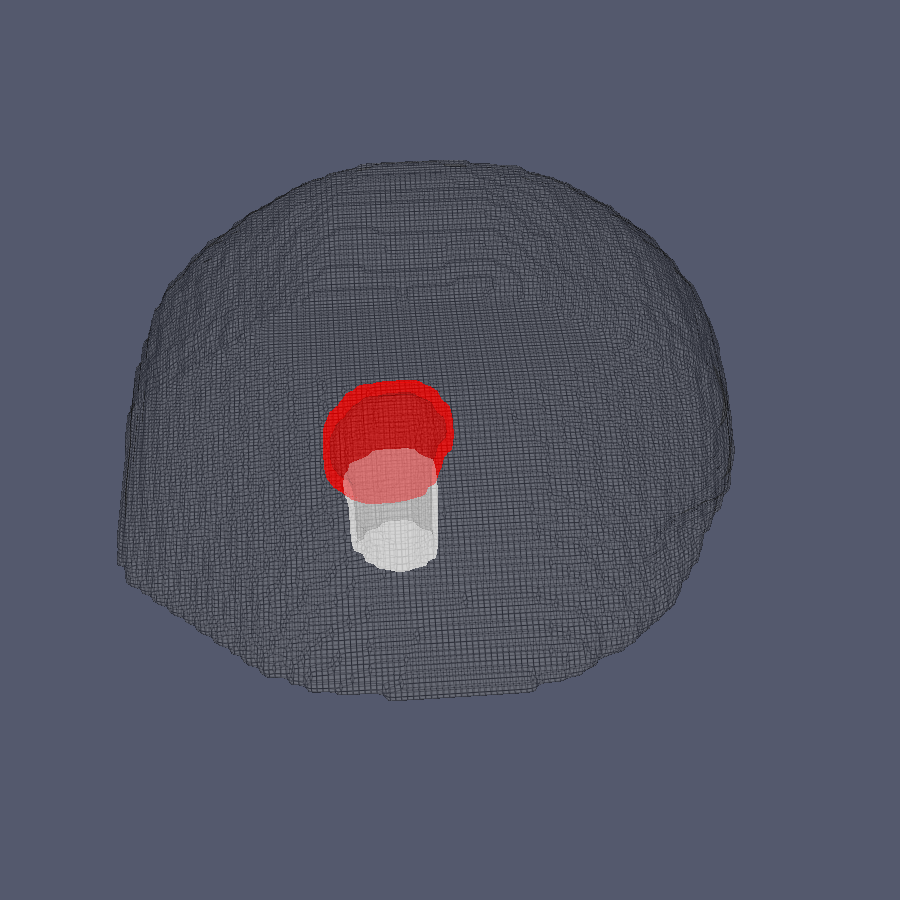
\includegraphics[width=\textwidth]{imgs/showcase_showcase_pred_8.png}
    \end{subfigure}
    \caption{Examples from the breast phantom data set. Blue is the background, the gray is the phantom surface, the red is the lump, and the white is the pillar used for holding the lump.}
    \label{fig:phantoms}
\end{figure}
\noindent In this work, I would like to use that data set to pursue one of the following tasks:
\begin{itemize}
    \item \textbf{Interpolating between real phantoms.} Rather than interpolating between two random noise vectors, we invert two real phantom volumes to recover their corresponding noise vectors, interpolate between these two latents, and integrate the ODE forward to generate the intermediate phantoms. We also explore interpolating between two random noise vectors and examine the resulting trajectory.

    \item \textbf{Sampling from fixed seeds across training checkpoints.} We fix a set of noise vectors and generate samples from them at several checkpoints during training (e.g., after 1k, 5k, 20k, and 50k steps). Arranging the outputs in rows lets us track how each sample evolves over the course of training. We expect the overall shape and position of the phantom to stabilize early, while fine texture and the boundaries of the lump and pillar settle later.

    \item \textbf{Checking the noise space.} Using ODE inversion, we map each of the approximately 800 phantom volumes to its corresponding noise vector. For a freshly sampled noise vector $z$, we generate the corresponding phantom $x$ and compare it to the phantoms whose latent codes are the $k$ nearest neighbors of $z$, measuring similarity only on the lump and pillar via per-class Dice score, centroid offset, and volume ratio. If generated samples resemble their latent neighbors more closely than they resemble randomly chosen phantoms, the noise space is locally coherent; otherwise, the mapping $z \to x$ is effectively arbitrary and nearby codes carry no shared meaning.
\end{itemize}


\end{document}
